\documentclass[11pt]{article}
\usepackage[T1]{fontenc}
\usepackage[margin=1in]{geometry}
\usepackage{amsmath,amssymb,amsthm,bm,graphicx,booktabs}
\usepackage[numbers,sort&compress]{natbib}
\usepackage[colorlinks=true,linkcolor=blue,citecolor=blue,urlcolor=blue]{hyperref}
\hypersetup{
 pdftitle={Query-Efficient Quantum Approximate Optimization via Graph-Conditioned Trust Regions},
 pdfauthor={Molena Huynh},
 pdfsubject={Quantum approximate optimization},
 pdfkeywords={QAOA, MaxCut, graph transfer, trust regions, finite-shot optimization}
}
\usepackage{microtype}
\usepackage{array}
\usepackage{placeins}
\usepackage{needspace}
\emergencystretch=1.5em
\setlength{\belowcaptionskip}{6pt}
\newcommand{\R}{\mathbb R}
\newcommand{\E}{\mathbb E}
\newcommand{\Prb}{\mathbb P}
\newcommand{\TV}{\operatorname{TV}}
\newcommand{\diag}{\operatorname{diag}}
\newcommand{\tr}{\operatorname{tr}}
\newcommand{\ket}[1]{\lvert #1\rangle}
\newcommand{\norm}[1]{\lVert #1\rVert}
\newtheorem{theorem}{Theorem}
\newtheorem{proposition}[theorem]{Proposition}
\newtheorem{corollary}[theorem]{Corollary}
\begin{document}
\raggedbottom
\title{Query-Efficient Quantum Approximate Optimization\\
via Graph-Conditioned Trust Regions}
\author{Molena Huynh\\
 \normalsize North Carolina State University\\
 \normalsize\href{mailto:Molena.Huynh@jmp.com}{\texttt{Molena.Huynh@jmp.com}}}
\date{}
\maketitle
\begin{abstract}
Parameter transfer can provide a useful starting point for the quantum
approximate optimization algorithm, but finite measurement budgets can
limit subsequent refinement. We formulate a graph-conditioned trust-region
policy for MaxCut that combines donor-derived geometry, sampled affine
models, radius-dependent shot allocation, and statistical acceptance tests.
The analysis connects local-model error to sufficient conditions for
affordable acceptance and distinguishes decision validity from detection
power. In ideal-circuit simulations, a 256-run experiment on 16 graphs
crosses sampling allocation with stopping after an unresolved test. All
four policies return identical parameters in 64 matched graph/depth/repetition
cases. Relative to
continuation that refits at the same radius, stopping reduces mean
optimization shots by 38--42\%; changing allocation produces no additional
quality improvement. A separate shape-by-rule experiment accepts four of
288 proposals, with smaller mean gains for the shaped policy than for
simultaneous perturbation stochastic approximation (SPSA) and constrained
optimization by linear approximation (COBYLA). Conditional diagnostics on eight additional graphs show
how model accuracy, proposal margin, and endpoint resolution jointly
determine accepted gain and measurement cost. These results establish
stopping-related savings within the tested policies and identify the
conditions limiting refinement. Predictions using exact simulator inputs
remain offline diagnostics; the study does not establish a general
optimization or query-complexity advantage from graph-conditioned geometry.
\end{abstract}

\section{Introduction}
The quantum approximate optimization algorithm (QAOA) optimizes an objective
over parameterized quantum states~\cite{farhi2014}. Even a shallow circuit
requires repeated measurements at each candidate parameter vector.
Transferring parameters from a related graph can provide a useful starting
point, but further refinement must produce improvements large enough to
resolve within the remaining measurement budget. We study this problem for
MaxCut, separating the quality inherited from transfer from the gain and
cost of subsequent optimization.

Parameter transfer is supported by interpolation and Fourier
initialization~\cite{zhou2020}, annealing-inspired schedules~\cite{sack2021},
concentration within specified random graph ensembles~\cite{brandao2018},
local subgraph structure and graph representations~\cite{galda2023,falla2024},
and precomputed tree angles~\cite{streif2020,wurtz2021}. Recent methods also
generate graph-conditioned trajectories~\cite{nguyen2026} or refine a
selected layer after transfer~\cite{patel2026}. These methods differ in
training, preprocessing, and online measurement costs. Initialization-only
controls are therefore necessary to identify the contribution of refinement.

Our proposed refinement policy combines a graph-selected initial vector,
called the anchor, with a fixed donor-derived region shape, an affine
interpolation model, and fresh endpoint measurements for acceptance.
Radius-dependent model sampling offsets the explicit inverse-radius factor
in the gradient-noise scale;
an unresolved acceptance test terminates the run. The policy, labeled
``RA'' (resolution-aware) in figures, is compared with its original version,
which contracts and continues after an unresolved test. An isotropic control
tests the chosen geometry, but separating graph-dependent orientation from
anisotropy would additionally require spectrum-matched random rotations.
We use circuit shots as the primary cost; an objective-estimation call and
a logical measurement batch are recorded separately.

The constituent numerical ideas have substantial precedent. QR-based
fitting and interpolation geometry control model
sensitivity~\cite{golub2013,conn2008}; local quadratic models and observation
reuse already improve variational optimizers~\cite{sung2020}, and ANASTAARS
uses noise-aware adaptive random subspaces~\cite{dzahini2025}. Shot allocation
is central to iCANS~\cite{kubler2020} and to spatial objective-and-variance
modeling for QAOA~\cite{ha2024}. Stochastic trust-region convergence theories
require accuracy and sampling conditions~\cite{chen2018,shashaani2018}
that the present finite-horizon policy does not enforce. Using an
empirical-Bernstein endpoint test does not reproduce those published
optimizers or establish an advantage over them.

We ask which components change the returned quality or measurement cost,
and when a useful model proposal can be resolved by its acceptance test.
Two factorial experiments separate region shape and confidence rule from
sampling allocation and unresolved stopping. Conditional diagnostics on
additional graphs connect model error, proposal margin, and accepted gain.
The analysis supplies explicit sufficient conditions and a policy-specific
power bound; the experiments determine their practical relevance. Exact
simulator inputs used for diagnosis are distinguished from information
available to the implemented optimizer.


\section{Graph-conditioned refinement and guarantees}
\label{sec:algorithm}
For a finite simple unweighted graph $G=(V,E)$ with $|E|>0$ at depth $p$,
minimize the normalized objective
$f_G=-F_G/|E|\in[-1,0]$, where $F_G$ is the expected cut and $d=2p$.
The default selector compares standardized degree and clustering descriptors
to choose an anchor $x_0$ from an offline bank. A regularized scatter matrix
of nearby, symmetry-aligned donor parameters defines a fixed symmetric
positive-definite shape $B$, with $\det B=1$ and
$\operatorname{cond}(BB^\top)\le4$; the isotropic control uses $B=I$.
The graph-dependent choices precede target optimization and use no
target-objective measurements.
An affine model $m(u)=\widehat c_0+\widehat c_{1:d}^{\top}u$ is fitted
at $d+1$ selected points in $x+\Delta B\{u:\|u\|_2\le1\}$.
The proposed direction uses the fitted gradient coefficients, whereas
fresh endpoint observations determine acceptance. For a proposal $u^+$,
write $q=m(0)-m(u^+)$ for predicted decrease, $a=f_G(x)-f_G(x^+)$
for true improvement, and $h=a-\eta q$ for its sufficient-decrease margin.
Appendix~\ref{sec:methods} specifies the interpolation geometry and
statistical assumptions; Appendix~\ref{sec:experimental-protocol} defines
the graph selector and shape construction. Model shots are fixed before each fit by
\begin{equation}
 S(\Delta)=\max\{2,\lceil S_0(\Delta_0/\Delta)^2\rceil\}.
 \label{eq:radiusshots}
\end{equation}

\Needspace{8\baselineskip}
\subsection{Resolution-aware refinement}
The resolution-aware routine \texttt{refine} takes an anchor $x_0$, a fixed shape
$B$, a shot cap $N_{\max}$, initial radius $\Delta_0$, initial model count
$S_0$, and prescribed acceptance looks, with $d=2p$. In the shape-by-rule experiment,
$(S_0,\Delta_0)=(256,0.1)$, $T=16$, $\eta=0.1$, $\alpha=0.05$, and
$s=(512,2048,8192,16384)$, with radius bounds $[0.025,0.8]$.
The input shape is $I$ or the bounded descriptor shape. Its output is the
last accepted incumbent, an explicit stopping reason, and the complete measurement record.
The cap covers optimization measurements; the 8192-shot independent output
evaluation is additional. Original-policy controls are specified in
Appendix~\ref{sec:experimental-protocol}.
\begin{enumerate}
\item Initialize $x=x_0$, $\Delta=\Delta_0$, and spent shots to zero.
Record the anchor as the incumbent at zero target-optimization shots;
reference-bank construction remains an offline cost. Seed separate streams for
classical point selection, model sampling, and endpoint sampling.
\item Before trial $t$, compute $S(\Delta)$ by Eq.~\eqref{eq:radiusshots}.
If the remaining shots cannot cover $(d+1)S(\Delta)+2s_1$, stop with
\texttt{resolution\_limited} and reason
\texttt{model\_and\_first\_look\_unaffordable}. Spend no model shots for
that untestable proposal. Reserving the first look assures feasibility of
one test; it does not assure detection at that look.
\item Select a full-rank QR design, sample its $d+1$ points at $S(\Delta)$,
and fit the affine model. Record radius, design, coefficients, shot count,
and condition number. If $q=\norm{\widehat c_{1:d}}_2<10^{-12}$, return
the incumbent with a flat-model resolution reason, retaining the model
shots already spent; this is not a stationarity test. Otherwise set
$u^+=-\widehat c_{1:d}/q$ and propose
$x^+=\operatorname{wrap}(x+\Delta Bu^+)$. The wrap operation applies
the exact angle periodicities specified in Appendix~\ref{sec:methods}.
\item At each prescribed look request fresh observations at both endpoints,
adding only $s_\ell-s_{\ell-1}$ samples per endpoint, with $s_0=0$.
If the next two-endpoint batch is unaffordable, consume none of it and mark
the trial unresolved for budget reasons. For an affordable look, compute
the decrease estimate $\widehat a_\ell$ and the interval
$[\widehat a_\ell-w_\ell,\widehat a_\ell+w_\ell]$, where
$w_\ell=2b_\ell$ for Eq.~\eqref{eq:bound}, or the sum of the two
endpoint radii for Eq.~\eqref{eq:bernstein}. Accept if its lower
endpoint is at least $\eta q$, and reject if its upper endpoint is below
$\eta q$. Otherwise continue to the next affordable look.
\item After acceptance set $x=x^+$, record its cumulative shot count, and
expand $\Delta$ by $1.5$ up to $0.8$. Only a certified rejection contracts the radius
to $\max\{0.5\Delta,0.025\}$. A rejection when already at the
radius floor terminates with
\texttt{radius\_limit}. An unresolved decision stops immediately with
\texttt{resolution\_limited}, recording whether stopping followed the final
prescribed look or an unaffordable batch; it leaves both the incumbent and radius
unchanged.
\item Count each attempted trial toward the declared horizon and continue unless
a stopping condition applies. Return the incumbent with status
\texttt{horizon} at horizon exhaustion, and return it at every other ordinary
stop. Rank failures or nonfinite inputs raise explicit errors; no substitute
model is used.
\end{enumerate}
This policy distinguishes insufficient measurement evidence from evidence
against sufficient decrease. A resolution stop means that the declared
model or decision schedule has ended without resolving a further update.
Other proposals, estimators, or allocations may still succeed. On the
simultaneous confidence event, a certified
rejection proves $h<0$, which still permits a positive improvement $a>0$.
The original \texttt{optimize} and \texttt{bernstein\_optimize} routines
contract after unresolved decisions. They are
used only for their explicitly labeled controls and replay.


\subsection{Finite-budget guarantees}
The analysis separates initialization, model accuracy, and the decision to
accept a proposal. Theorem~\ref{thm:transfer} bounds objective discrepancy
by total variation between rooted edge-neighborhood distributions and,
given an $\epsilon$-optimal donor on a common parameter domain, bounds
transferred regret. Disjoint neighborhood-type distributions give only the
objective-range bound. This structural certificate does not justify the
descriptor selector or the orientation of the donor-derived shape.

Proposition~\ref{prop:model} bounds affine coefficient error by
$\mathcal E$, separating Taylor remainder from amplified measurement noise.
Proposition~\ref{prop:biasvariance} gives the conditional bias--variance
identity for the physical-gradient fitting map. For fixed design and shape,
inverse-square allocation stabilizes the leading gradient-noise scale;
it neither makes that error vanish nor guarantees a useful direction.
These statements motivate the radius diagnostics, rather than certify
each executed model.

Theorem~\ref{thm:acceptance} gives the decision guarantee: with probability
at least $1-\alpha$, every accepted step in the adaptive finite horizon
has true decrease at least $\eta q>0$. Validity alone does not assure
acceptance. The following sufficient condition connects model error,
endpoint resolution, and the total cost of one update. For final cumulative
count $s_L$ per endpoint and $L$ prescribed looks, write
$b_L=\sqrt{\log(4TL/\alpha)/(2s_L)}$.

\begin{corollary}[Sufficient model accuracy and budget for acceptance]
\label{cor:modelacceptance}
Under the hypotheses of Proposition~\ref{prop:model} and
Theorem~\ref{thm:acceptance}, consider
at most $T$ trials. For $\delta\in(0,1)$, use $\delta/T$ in each trial's
Eq.~\eqref{eq:modelerror}, with resulting bound $\mathcal E$ and a valid
trial-region gradient-Lipschitz constant $L_f$. Let $N_{\rm rem}$ be the
budget before model measurements and $N_{\rm model}$ their cost, equal to
$(d+1)S(\Delta)$ for the implemented square design. With probability at
least $1-\delta-\alpha$, the following implication holds simultaneously
at every executed nonflat trial, with $q\ge10^{-12}$ and
$u^+=-\widehat c_{1:d}/q$: if
\begin{equation}
 \begin{aligned}
 (1-\eta)q&\ge\mathcal E+\tfrac12L_f\Delta^2\norm{Bu^+}_2^2+4b_L,\\
 N_{\rm model}+2s_L&\le N_{\rm rem},
 \end{aligned}
 \label{eq:modelacceptance}
\end{equation}
then the Hoeffding rule accepts by the final look, provided unresolved
trials proceed through the prescribed looks whenever affordable.
\end{corollary}

The fitted intercept cancels in the predicted decrease, leaving one
coefficient-error allowance and one Taylor remainder. The statement is a
simultaneous implication on the confidence events; it is not a coverage
guarantee conditional on selecting models that satisfy the random
inequality. The policy estimates neither $L_f$ nor $\mathcal E$ and does
not enforce this sufficient certificate. Proposition~\ref{prop:acceptancepower}
separately bounds the probability that the specified Hoeffding rule accepts
a small-margin proposal. Full proofs and the empirical-Bernstein extension
are in Appendix~\ref{sec:methods}. These results connect accuracy to
affordable decisions without establishing a general optimization or
query-complexity advantage.


\section{Results}
The main comparisons use unweighted MaxCut instances with 12 or 14 vertices,
depths $p=2,3$, and ideal computational-basis measurements simulated from
the exact cut distribution. Optimizer outcomes are evaluated by exact
expectations at the returned parameters. Optimization-shot counts include
unsuccessful attempts; each returned optimizer output also incurs 8192 independent
evaluation shots, reported separately. Optimizer intervals are descriptive
pointwise 95\% graph-bootstrap intervals after averaging measurement
repetitions within each graph, conditional on the two fixed reference banks.
Diagnostic captions distinguish graph uncertainty from conditional Monte
Carlo uncertainty. Appendix~\ref{sec:experimental-protocol} gives the
sampling protocols, costs, and uncertainty calculations.

\subsection{Quality at a measured shot budget}
\label{sec:empirical}
We measure refinement by the gain over each policy's own anchor,
$I_G=100[f_G(\theta_0)-f_G(\theta_{\rm out})]$, in percentage points.
The complementary signed deficit
$D_G=100[f_G(\theta_{\rm out})-f_G^{\rm ref}]$ uses a best-found,
uncertified reference. The shape-by-rule experiment comprises 256 runs on
16 previously examined targets, two fixed banks, depths two and three,
and a 65,536-shot optimization cap. It is a post hoc comparison with
matched anchors and previously selected settings. The conventional
comparators are simultaneous perturbation stochastic approximation (SPSA)
and constrained optimization by linear approximation (COBYLA).
The shaped resolution-aware Bernstein policy gains 0.065 and 0.032
percentage points at the two depths, compared with 0.196 and 0.359 for
SPSA and 0.083 and 0.197 for COBYLA. COBYLA also uses fewer mean shots.
The paired gain differences from SPSA are $-0.13$ (95\% interval
$-0.21$ to $-0.05$) and $-0.33$ ($-0.47$ to $-0.20$) percentage points.
Figure~\ref{fig:efficiency} retains initialization at zero shots and follows
each available output through completed measurement batches. These
trajectories quantify the observed cost--quality tradeoff.
The paired analysis and measurement accounting are specified in
Appendix~\ref{sec:experimental-protocol}.

\begin{figure}[!htbp]
\centering
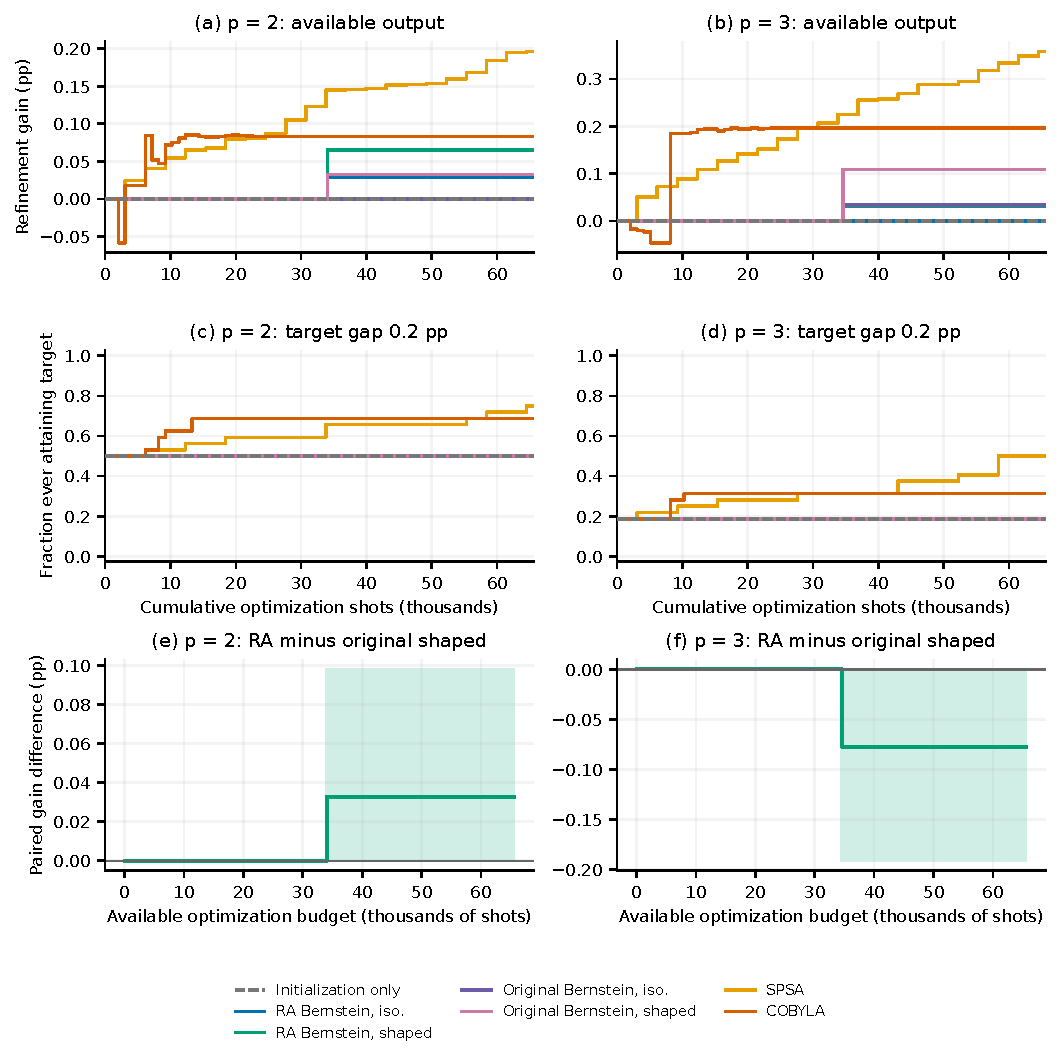
\includegraphics[width=\textwidth]{figures/efficiency.pdf}
\caption{Solution quality versus measurement expenditure. RA denotes
resolution-aware refinement. Step lines use
the last recorded incumbent available at each cumulative optimization-shot
budget. Until a sampling batch is complete, the preceding incumbent remains
available. The anchor appears at zero shots. Target-attainment curves retain
every run and count initial successes at zero shots. The target,
$f_G^{\mathrm{ref}}+0.002$, was fixed before the resolution-aware experiment.
Exact expectations evaluate recorded outputs retrospectively; they do not
select them. Each trajectory comes from a run at one cap, rather than
interpolation between separate runs with different caps.
Pointwise 95\% bands resample whole graph trajectories within the two fixed
panels, each containing eight graphs with two measurement repetitions per
graph and depth. Gains are in percentage points. The third row shows the paired gain difference between resolution-aware
and original shaped Bernstein. Flat tails indicate that the returned output
remains available after termination without further expenditure. First
attainment does not imply continued satisfaction of the target for a
nonmonotone baseline.}
\label{fig:efficiency}
\end{figure}

\subsection{Stopping accounts for the savings}
The separate sampling-by-stopping factorial crosses fixed or
radius-dependent model shots with stopping or refitting after an unresolved
test. It contains 256 shaped Bernstein runs on the same 16 targets.
All four policies return identical vectors in the 64 matched
graph/depth/repetition cases. With fixed model shots, stopping reduces
mean expenditure by 39.76\% (95\% graph interval 34.65--44.02\%) at
depth two and 41.74\% (36.17--46.43\%) at depth three; the corresponding
radius-dependent savings are 38.32\% and 40.40\%.
Figure~\ref{fig:attribution} attributes these savings to termination,
with no returned-quality gain from the allocation intervention. The
continuation control retains its radius, whereas the original policy
contracts it. The shared cap also restricts continuation: two complete
endpoint tests alone cost 65,536 shots, leaving nothing for their models.
These comparisons therefore do not identify the best use of residual budget.
The figure's calibration panels concern a separate fresh-graph diagnostic,
described below and in Appendix~\ref{sec:joint-protocol}.

\begin{figure}[!htbp]
\centering
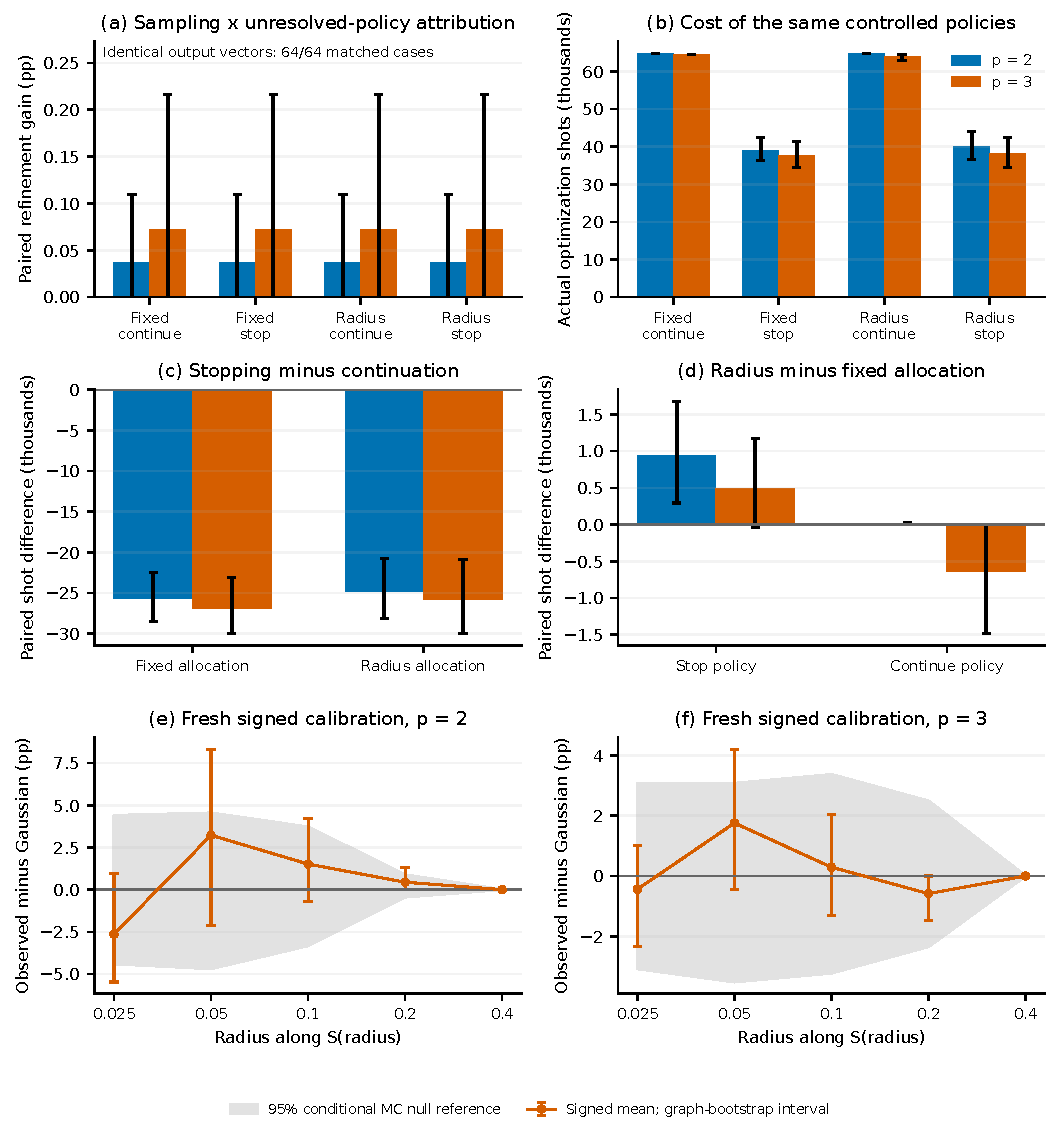
\includegraphics[width=\textwidth]{figures/attribution.pdf}
\caption{Attribution of expenditure and calibration residuals. Grouped bars
report own-anchor gain and optimization shots for the four
sampling-by-stopping policies; all four return identical parameter vectors
in the 64 matched cases. Paired contrasts show stop minus continue and
radius-dependent minus fixed allocation, with negative cost differences
indicating savings. Continuation refits at the same radius after an unresolved
test. Bottom panels show fresh-graph observed minus Gaussian-predicted
positive-margin frequency. Pointwise 95\% graph-bootstrap intervals describe variation
across the eight targets conditional on their fixed reference bank. A
separate conditional Monte Carlo reference quantifies frequency-estimation
noise in 32 sampled-model and 256 Gaussian proposals per condition, assuming
equal underlying probabilities within each condition. The reference is not
a bound on Gaussian approximation error. All intervals are pointwise.}
\label{fig:attribution}
\end{figure}

\subsection{Radius trades bias against noise}
Figure~\ref{fig:components} evaluates the model on the original eight-graph
diagnostic panel. At fixed shot count, contraction amplifies physical-gradient
noise through the radius-dependent fitting map. Increasing the shot count
reduces this sampling term but leaves finite-radius affine bias.
The implemented inverse-square schedule approximately stabilizes the
explicit variance prefactor, while smaller radii increase model cost.
Equation~\eqref{eq:biasvariance} separates these
effects, using exact simulator inputs for prediction. Its numerical
calibration tests the fixed linear fitting map under the ideal observation
model; an online total-error prediction would additionally require measured
variance information and estimates or valid bounds for model bias.
Only 31 of the 256 shape-by-rule runs fit a model at a changed radius,
which limits what that optimizer experiment alone can establish about
the allocation schedule.

\begin{figure}[!htbp]
\centering
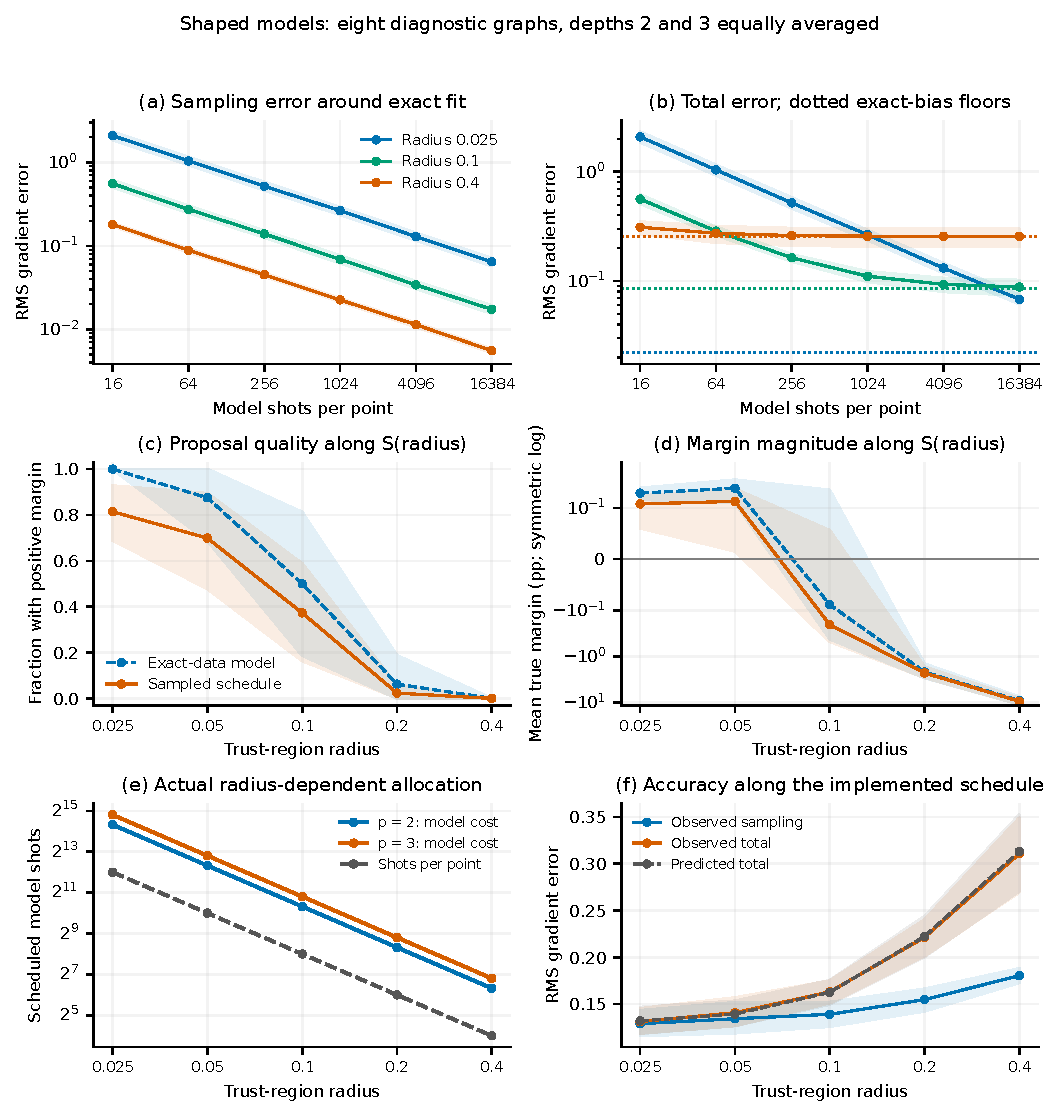
\includegraphics[width=0.95\textwidth]{figures/components.pdf}
\caption{Radius, model bias, and propagated shot noise. Lines report root-mean-square (RMS)
sampling error about an exact-data affine gradient, RMS total error against
a numerically checked exact-objective gradient, and the exact-data bias
floor. The plotted models use the donor-derived shape. Gradient errors
are in inverse radians, and radii are in radians. Radius panels show both
positive-margin frequency and true margin
magnitude; the margin axis is symmetric logarithmic with a linear region
around zero. The allocation panels evaluate $S(\Delta)$, including 64 and
16 shots at radii 0.2 and 0.4, and distinguish model expenditure from error.
The diagnostic population comprises the eight graphs in the first follow-up
panel. Depths two
and three are aggregated with equal graph weights as stated in the panels.
RMS panels use 128 sampled fits per condition; margin-frequency panels use
32 sampled proposals per condition. Pointwise 95\% bands resample graphs
rather than treating repeated fits as new
graphs. Predicted errors use the conditional variance-propagation identity
with exact simulator inputs.}
\label{fig:components}
\end{figure}

\subsection{Valid tests can have little power}
The 288 shape-by-rule proposals contain 178 nonimproving points,
30 improving points without positive sufficient-decrease margin,
76 positive-margin points left unresolved, and four accepted improvements.
These are dependent proposals, not independent graphs. Separately,
Fig.~\ref{fig:acceptance-power} fixes 160 diagnostic proposals and repeats
their endpoint measurements. On its positive-margin cohort, the online
four-look Bernstein rule accepts with mean frequency 0.0233
(pointwise replay interval 0.0075--0.0391) at the 32,768-shot pair cap;
the mean unresolved fraction is 0.9767. The five-look extension is a
different confidence schedule. Zero acceptances in 128 replays of one
proposal imply a one-sided 95\% upper limit of about 2.31\%, so this
experiment cannot validate the much smaller analytical bound in
Proposition~\ref{prop:acceptancepower}. The replay measures conditional
power, not the success probability of a complete optimizer.

\begin{figure}[!htbp]
\centering
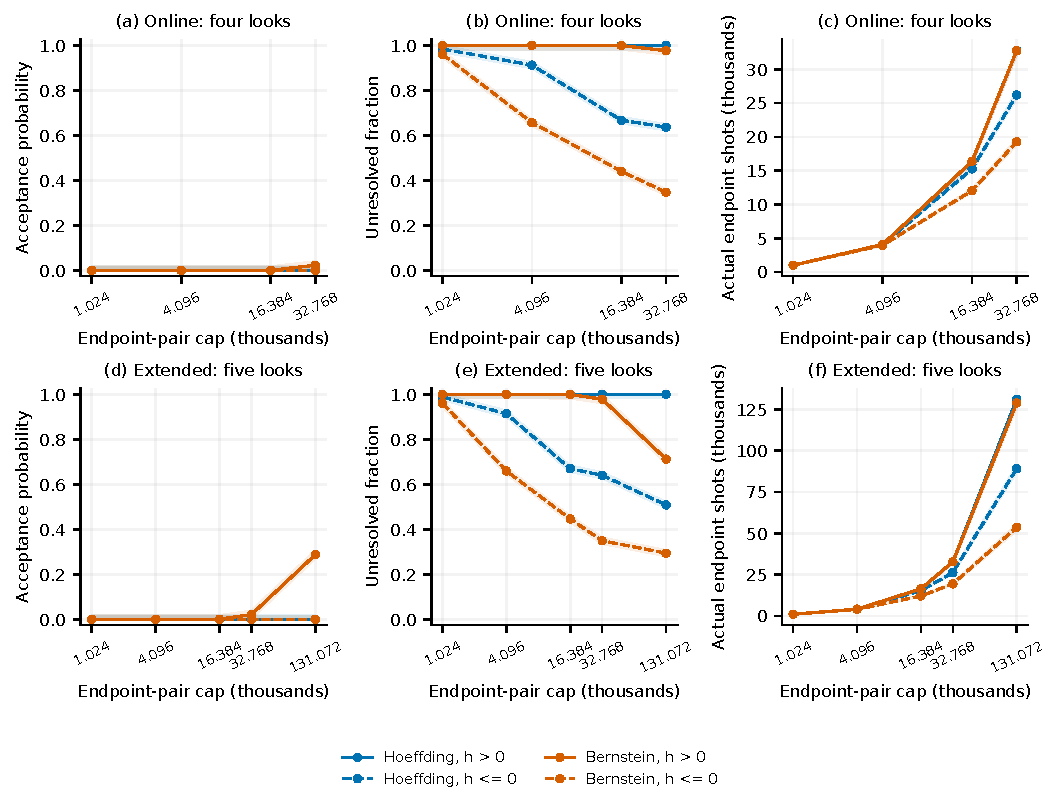
\includegraphics[width=\textwidth]{figures/acceptance_power.pdf}
\caption{Acceptance power versus endpoint-pair budget. The 160 fixed
diagnostic proposals use 1024 model shots per point and have equal weights
within each cohort at every budget: 58 have positive margin and 102 have
nonpositive margin. The curves estimate conditional replay
power, rather than acceptance frequencies along optimizer trajectories.
The first row uses
the online four-look schedule and its $L=4$ confidence penalty; the second
uses the separately labeled five-look extension. Panels report acceptance
probability, unresolved fraction, and endpoint expenditure, retaining
unresolved cases at their last affordable look. Lines distinguish Hoeffding
and Bernstein within fixed positive-margin and nonpositive-margin cohorts.
Bands are conservative pointwise 95\% Hoeffding bounds for the fixed-cohort
replay means, conditional on these proposals. There are 128 replays per proposal;
zero acceptances for one proposal give a one-sided 95\% binomial upper limit
of $1-0.05^{1/128}\simeq2.31\%$. This resolution cannot establish zero
power or validate a probability near $10^{-6}$. Budgets are plotted on a
base-two logarithmic axis. The online acceptance panel uses a 0--0.06
vertical range to resolve low power; its extension has a separate scale.
This fixed-$S=1024$ population does not implement the radius-dependent
model allocation tested in Fig.~\ref{fig:joint-utility}.}
\label{fig:acceptance-power}
\end{figure}

\subsection{From proposal margin to accepted gain}
\label{sec:joint-results}
Figure~\ref{fig:joint-utility} follows proposals on eight additional graphs
through the implemented allocation and four-look decision schedule.
All failed attempts remain in the gain and cost averages. At depth three,
radius 0.1 gives a sampled Bernstein mean accepted gain of 0.180
percentage points (95\% graph interval 0.000--0.471), concentrated on
two of eight graphs, at a mean model-plus-endpoint cost of 33,336 shots.
Radius 0.025 gives no accepted gain and costs 61,440 shots per attempt.
Thus a high positive-margin frequency need not yield the greatest accepted
gain. This diagnostic evaluates one attempted step from each fixed anchor,
with repeated model and endpoint draws; it is not an
optimizer benchmark or a radius-selection procedure.

The Gaussian prediction uses exact target means, variances, and trial
objectives. Across all 80 fresh shaped graph/depth/radius conditions,
its mean absolute positive-margin frequency difference is 2.02 percentage
points (95\% graph interval 1.45--2.52). This point estimate lies within
the separate conditional Monte Carlo reference range, 1.65--2.78
percentage points, at the available simulation resolution.
The radius/depth lookup controls have less target information, so their
larger errors do not establish an online efficiency advantage. Graph
intervals and Monte Carlo references answer different uncertainty questions;
neither isolates Gaussian approximation error. The full protocol preserves
all outcomes and charges model and endpoint measurements separately from
the offline exact-simulation cost.

\begin{figure}[!htbp]
\centering
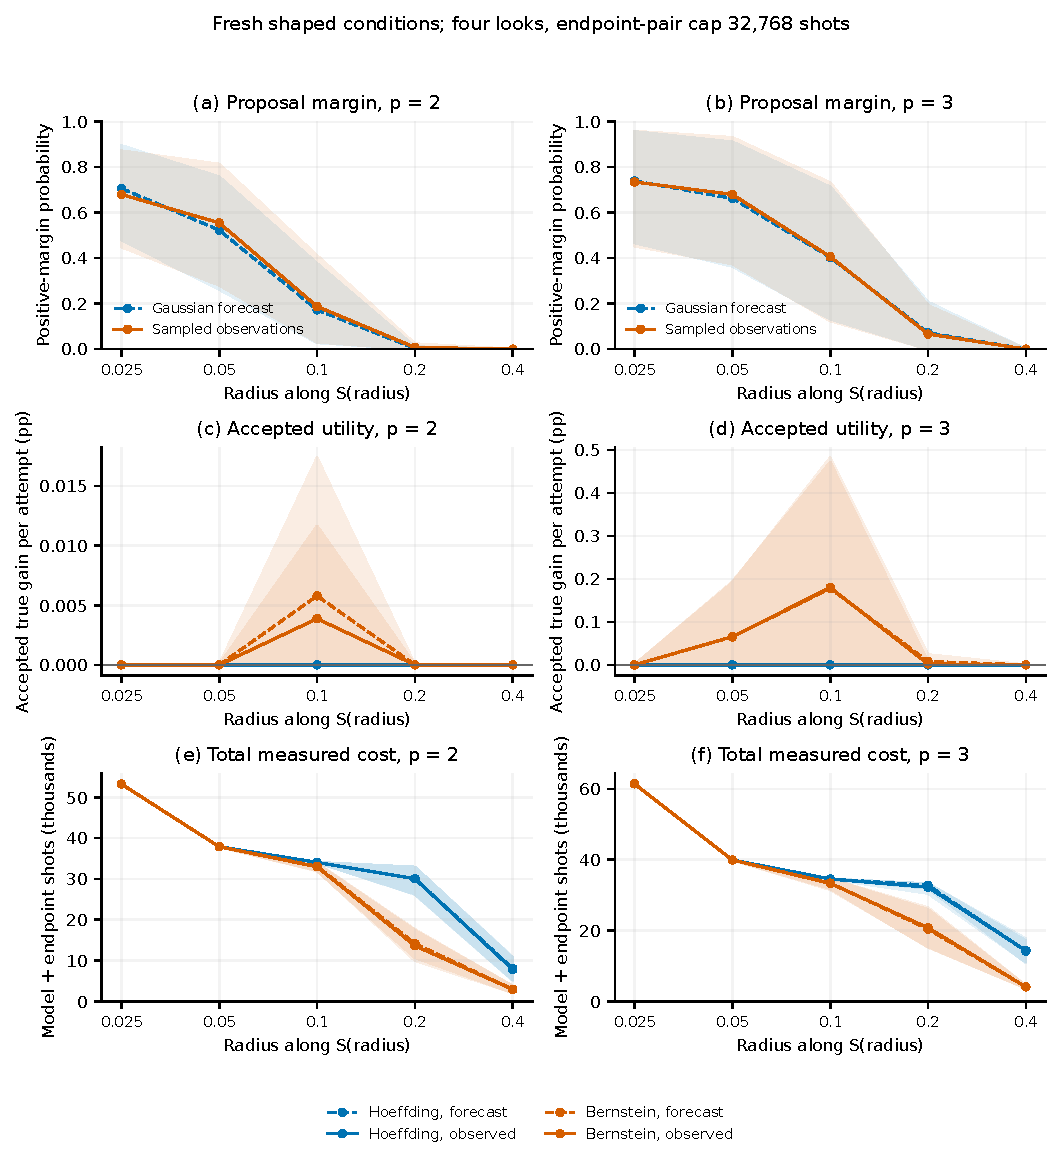
\includegraphics[width=0.86\textwidth]{figures/decision.pdf}
\caption{Proposal quality and decision cost on the same allocation schedule
for eight fresh graphs with a fixed reference bank. Columns show depths two
and three. Rows show positive-margin probability,
accepted true gain including zero outcomes, and model-plus-endpoint shots versus
radius. Scheduled per-point counts are 4096, 1024, 256, 64, and 16 at radii
0.025, 0.05, 0.1, 0.2, and 0.4. Top panels include radius-only and
radius-plus-depth predictors fitted to the eight original graphs; their
training set is fixed. Information access is unequal: the Gaussian
forecast uses exact fresh-target moments and trial objectives, making it
an offline diagnostic. Each fresh shaped condition supplies 32 sampled
proposals with eight endpoint replays each, versus 256 Gaussian proposals
with one replay each. Both confidence rules share endpoint streams, the
online $L=4$ penalty, and a 65,536-shot cap. Lines average graphs equally;
pointwise 95\% bands resample whole graphs for observed and Gaussian curves.
The fixed lookup curves have no bands. The probability curves average
predictions before comparison, whereas Eq.~\eqref{eq:probabilitymae}
averages absolute errors within individual conditions. Every proposal
remains in the denominator, including nonimproving,
rejected, and unresolved attempts.}
\label{fig:joint-utility}
\end{figure}


\section{Discussion}
Stopping unresolved tests reduces measurement expenditure under the
specified continuation policy. Identical outputs across the
sampling-by-stopping experiment exclude improved quality from
radius-dependent allocation as the source of these savings. The
shape-by-rule comparison shows a quality--cost tradeoff, with larger mean
gains for conventional baselines. The evidence supports this specific
stopping benefit without establishing general optimizer superiority.

Contraction can reduce affine bias while amplifying gradient noise at
fixed shot count and shrinking the proposed improvement.
Corollary~\ref{cor:modelacceptance} connects model accuracy to affordable
acceptance, but the optimizer does not enforce its condition. Exact-moment
calibration checks a standard linear-estimation identity; the Gaussian
forecast tests the nonlinear proposal map using additional target
information. Neither supplies a controller using measured inputs. The
joint diagnostic concerns one attempted step from a fixed anchor.

Isotropic and shaped comparisons leave the contribution of graph-dependent
orientation unresolved. Fixing anchors and eigenvalue spectra while varying
orientation would separate it from initialization and anisotropy. An
operational controller requires accessible estimates or valid bounds,
an allocation rule, and charged pilot measurements. Relevant comparators
include spatial objective-and-variance modeling~\cite{ha2024} and
time-uniform confidence sequences~\cite{howard2021}, which change model
construction and sampling or replace prescribed looks. Changing the
endpoint rule alone does not reproduce either approach.

The 16 optimizer targets were previously examined; eight additional graphs
test a conditional mechanism with a fixed bank. Measurement repetitions
are not independent graphs, and banks are not crossed with common targets.
Small-graph, ideal-circuit experiments leave device noise, drift, routing,
and hardware latency untested. The finite horizon, positive radius floor,
and absence of fully linear model guarantees preclude general convergence
or query-complexity claims. The open question is whether a practical
graph-conditioned controller can produce affordable, reproducible
improvements across independent problem regimes.

\FloatBarrier
\appendix
\section{Mathematical guarantees}
\label{sec:methods}

\subsection{Objective, observations, and local coordinates}
For a finite simple unweighted graph $G=(V,E)$ with $n=|V|$ and
$m=|E|>0$, define $C_G=\sum_{(i,j)\in E}(I-Z_iZ_j)/2$ and
$H_X=\sum_{i\in V}X_i$. At integer depth $p\ge1$, with
$\theta=(\gamma_1,\ldots,\gamma_p,\beta_1,\ldots,\beta_p)$,
\begin{equation}
 \ket{\psi_G(\theta)}=
 e^{-i\beta_pH_X}e^{-i\gamma_p C_G}\cdots
 e^{-i\beta_1H_X}e^{-i\gamma_1 C_G}\ket{+}^{\otimes n},
 \qquad f_G(\theta)=-\langle C_G\rangle_\theta/m.
 \label{eq:state}
\end{equation}
One computational-basis observation is $Y=-C_G(z)/m\in[-1,0]$,
with mean $f_G(\theta)$. The ideal simulator draws batches from the exact
cut-value distribution and charges every represented measurement.
The analysis assumes fresh conditionally independent shots at each sampled
point; the empirical-Bernstein extension additionally assumes identical
conditional distributions within each endpoint stream.

The objective has coordinate periods $2\pi$ for $\gamma_j$ and $\pi/2$
for $\beta_j$. The former follows from the integer cut spectrum; the latter
from the global bit flip commuting with the circuit and preserving the
initial state up to phase. Simultaneous reversal of all angles preserves
the objective by complex conjugation. The operation $\operatorname{wrap}$
uses the coordinate periods. Local models use the unwrapped region
\begin{equation}
 \mathcal T(x,\Delta,B)=\{x+\Delta Bu:\norm u_2\le1\},
 \qquad \Delta>0,\quad B=B^\top\succ0,\quad\det B=1,
 \label{eq:region}
\end{equation}
with $d=2p$. Wrapping leaves its objective values unchanged. The fixed shape
preserves region volume at a given radius; this does not imply useful
alignment with the objective.

\subsection{Transfer through rooted neighborhoods}
Let $\mu_{G,p}$ be the distribution of rooted isomorphism types obtained
by sampling an edge uniformly and taking the induced subgraph on vertices
within distance $p$ of either endpoint, marked as an unordered root pair.

\begin{theorem}[Transfer through rooted edge neighborhoods]
\label{thm:transfer}
For two finite simple unweighted graphs with at least one edge at a shared
depth $p$, let $d_p(G,H)=\TV(\mu_{G,p},\mu_{H,p})$, where
$\TV(\mu,\nu)=\tfrac12\sum_\tau|\mu(\tau)-\nu(\tau)|$. Then
\begin{equation}
 \sup_{\theta\in\R^{2p}}|f_G(\theta)-f_H(\theta)|\le d_p(G,H).
 \label{eq:transfer}
\end{equation}
If $\Omega\subseteq\R^{2p}$ is nonempty, $\theta_H\in\Omega$, and
$f_H(\theta_H)\le\inf_{\theta\in\Omega}f_H(\theta)+\epsilon$ for
$\epsilon\ge0$, then
\begin{equation}
 0\le f_G(\theta_H)-\inf_{\theta\in\Omega}f_G(\theta)
 \le\min\{1,\epsilon+2d_p(G,H)\}.
 \label{eq:transferregret}
\end{equation}
\end{theorem}
\begin{proof}
Propagate $C_e=(I-Z_uZ_v)/2$ backwards through the depth-$p$ circuit.
A mixer cannot enlarge support. Within each commuting cost layer, every
gate disjoint from the pre-layer support cancels; the remaining gates add
only immediate neighbors. Thus the expectation depends only on the
radius-$p$ edge neighborhood~\cite{farhi2014,brandao2018}. Extra outer-boundary
edges may be irrelevant, so this representation is sufficient rather than
minimal. Root-preserving isomorphism, uniform angles, and the product
initial state give a common response $h_p(\tau,\theta)\in[0,1]$ with
$-f_G(\theta)=\sum_\tau\mu_{G,p}(\tau)h_p(\tau,\theta)$.
The total-variation bound for expectations of $[0,1]$-valued functions
proves Eq.~\eqref{eq:transfer}. Furthermore,
$f_G(\theta_H)\le f_H(\theta_H)+d_p$ and
$\inf_\Omega f_H\le\inf_\Omega f_G+d_p$.
The assumed donor gap gives $\epsilon+2d_p$; membership in $\Omega$
and the objective range give the lower bound zero and upper bound one.
\end{proof}
Disjoint type distributions have $d_p=1$, yielding only the objective-range
bound. Multistart local minimization does not certify the donor gap
$\epsilon$. This certificate concerns rooted-neighborhood TV, not the
descriptor selector, global transport score, or donor-derived shape.

\subsection{Affine model accuracy and propagated variance}
For local points $u_i$, let $A_i=(1,u_i^\top)$ and
$m(u)=\widehat c_0+\widehat c_{1:d}^\top u$. The sample means $y_i$
use $S_i$ observations, with $W=\diag(S_i)$ and thin factorization
$W^{1/2}A=QR$. A full-rank weighted fit is
$\widehat c=R^{-1}Q^\top W^{1/2}y$. Writing $y=Ac^*+r+e$ gives
\begin{equation}
 \widehat c-c^*=R^{-1}Q^\top W^{1/2}(r+e).
 \label{eq:qridentity}
\end{equation}
Here $c^*$ contains Taylor coefficients, $r$ is the Taylor remainder at
the design points, and $e$ is sample-mean error. The implemented square
$N=d+1$ design interpolates $y$: its coefficient map is $A^{-1}$, regardless
of positive weights. QR solves evaluate the fit without forming normal equations.

The implemented design draws $d+1$ independent standard Gaussian vectors
and normalizes them to the unit sphere, then adds $0$ and the signed
coordinate vectors $\pm e_j$. Column-pivoted QR~\cite{businger1965} of the
transposed candidate design selects $d+1$ rows. Only selected points incur
measurements; no objective observation enters selection. A full-rank check
precedes fitting. We do not establish a uniform quantitative lower bound on
$\sigma_{\min}(R)$ or optimality of the selected set.

\begin{proposition}[Local model error with bounded observations]
\label{prop:model}
Suppose $\nabla f$ is $L_f$-Lipschitz on a convex set containing
$\mathcal T(x,\Delta,B)$. Choose $N\ge d+1$ points with $\norm{u_i}_2\le1$
and integers $S_i\ge1$ before drawing independent observations in
$[-1,0]$ with mean $f(x+\Delta Bu_i)$ at point $i$.
Assume $W^{1/2}A=QR$ has full column rank, and set
$c^*=(f(x),\Delta B^\top\nabla f(x))^\top$,
$a_i=L_f\Delta^2\norm{Bu_i}_2^2/2$, and $\sigma=\sigma_{\min}(R)>0$.
For $\delta\in(0,1)$, with probability at least $1-\delta$,
\begin{equation}
 \norm{\widehat c-c^*}_2\le
 \frac{\sqrt{\sum_i S_i a_i^2}+\sqrt{\tfrac N2\log(2N/\delta)}}{\sigma}
 =:\mathcal E,
 \label{eq:modelerror}
\end{equation}
and, on the same event, uniformly for $\norm u_2\le1$,
\begin{equation}
 |f(x+\Delta Bu)-m(u)|
 \le\tfrac12L_f\Delta^2\norm B_2^2+\sqrt2\,\mathcal E.
 \label{eq:uniformmodel}
\end{equation}
The statements hold conditionally when the region, design, and shot counts
are chosen from the preceding history and the sampling assumptions hold
conditional on that history.
\end{proposition}
\begin{proof}
Taylor's theorem gives $|r_i|\le a_i$. Hoeffding's inequality~\cite{hoeffding1963}
and a union bound give $|e_i|\le\sqrt{\log(2N/\delta)/(2S_i)}$ for all
$i$ with probability at least $1-\delta$. Consequently,
$\norm{W^{1/2}r}_2\le\sqrt{\sum_iS_i a_i^2}$ and
$\norm{W^{1/2}e}_2\le\sqrt{N\log(2N/\delta)/2}$.
Equation~\eqref{eq:qridentity} and
$\norm{R^{-1}Q^\top}_2=1/\sigma$ prove Eq.~\eqref{eq:modelerror}.
At an arbitrary $u$, the Taylor remainder is at most
$L_f\Delta^2\norm B_2^2/2$ and $\norm{(1,u^\top)}_2\le\sqrt2$, proving
Eq.~\eqref{eq:uniformmodel}. Conditioning fixes the region and sampling
choices before the observations, so the same argument applies.
\end{proof}

Let $\mathcal H$ contain all choices preceding the model measurements.
Conditionally, put $\bar y_i=f(x+\Delta Bu_i)$ and
$v_i=\operatorname{Var}(Y_i\mid\mathcal H)$. Independent streams with
independent shots of variance $v_i$ within point $i$ give
$\E[e\mid\mathcal H]=0$ and $\Sigma_y=\diag(v_i/S_i)$.
With $P=(0,I_d)$, define
\begin{equation}
 L_A=\Delta^{-1}B^{-\top}P R^{-1}Q^\top W^{1/2},\qquad
 \widehat g=L_Ay,\quad\bar g=L_A\bar y,\quad g=\nabla f(x).
 \label{eq:gradientmap}
\end{equation}
\begin{proposition}[Conditional gradient mean-square error]
\label{prop:biasvariance}
Under the stated conditional unbiasedness and finite-variance assumptions,
\begin{equation}
 \E[\norm{\widehat g-g}_2^2\mid\mathcal H]
 =\norm{\bar g-g}_2^2+\tr(L_A\Sigma_yL_A^\top).
 \label{eq:biasvariance}
\end{equation}
Replacing $g$ with $\bar g$ leaves only the trace term.
\end{proposition}
\begin{proof}
Expand $\widehat g-g=(\bar g-g)+L_Ae$. Conditional unbiasedness eliminates
the cross term, and
$\E[e^\top L_A^\top L_Ae\mid\mathcal H]=\tr(L_A\Sigma_yL_A^\top)$.
\end{proof}
This is the standard identity for a fixed linear estimator. Exact simulator
moments supply its offline diagnostic inputs. For equal counts and fixed
design and shape, gradient sampling error scales as
$\Delta^{-1}S^{-1/2}$: Eq.~\eqref{eq:radiusshots} stabilizes this leading
scale, whereas $S\propto\Delta^{-4}$ is sufficient for an $O(\Delta)$
noise bound, apart from confidence factors. Neither statement removes
Taylor bias or guarantees a useful direction. Full rank alone supplies no
uniform design bound, and the implementation does not estimate $L_f$ or
enforce a fully linear model condition~\cite{conn2008,chen2018,shashaani2018}.

\subsection{Independent acceptance and finite-budget detection}
For a nonflat model, $q=\norm{\widehat c_{1:d}}_2\ge10^{-12}$,
$u^+=-\widehat c_{1:d}/q$, and $x^+=\operatorname{wrap}(x+\Delta Bu^+)$.
Thus $q=m(0)-m(u^+)$, $a=f_G(x)-f_G(x^+)$, and $h=a-\eta q$.
Fix integers $T,L\ge1$, $0<\alpha,\eta<1$, and cumulative integer
looks $1\le s_1<\cdots<s_L$ before the run. Fresh endpoint streams give
\begin{equation}
 b_\ell=\sqrt{\frac{\log(4TL/\alpha)}{2s_\ell}},\qquad
 \widehat a_\ell=\overline Y_{x,\ell}-\overline Y_{+,\ell}.
 \label{eq:bound}
\end{equation}
The Hoeffding rule accepts if
\begin{equation}
 \widehat a_\ell-2b_\ell\ge\eta q,
 \label{eq:accept}
\end{equation}
rejects if $\widehat a_\ell+2b_\ell<\eta q$, and otherwise remains unresolved.
Later looks add only the difference in cumulative counts. Omitted or
unaffordable paired batches consume no shots.

\begin{theorem}[Simultaneous validity over prescribed looks]
\label{thm:acceptance}
Consider at most $T$ adaptive trials. Conditional on the history before a
trial's endpoint measurements, fix its center, proposal, and $q>0$, then
start fresh streams of conditionally independent observations in $[-1,0]$
with the corresponding true objective means. At the prescribed looks,
with probability at least $1-\alpha$, every executed endpoint interval
is valid and every acceptance satisfies $a\ge\eta q>0$.
Early stopping and budget-based omission of looks preserve this guarantee.
\end{theorem}
\begin{proof}
For one endpoint and look, conditional Hoeffding failure probability is
$2\exp(-2s_\ell b_\ell^2)=\alpha/(2TL)$. Union bounding two endpoints
and $L$ looks gives at most $\alpha/T$ per trial. Taking expectations and
union bounding at most $T$ trials gives $\alpha$. Cumulative looks may
share observations; their independence is unnecessary. On this event,
$|\widehat a_\ell-a|\le2b_\ell$, so Eq.~\eqref{eq:accept} gives
$a\ge\eta q$. Stopping only removes controlled events.
\end{proof}
The guarantee is per run and requires no accurate local model. On the same
event, rejection proves $h<0$, which can still accompany $a>0$; an unresolved
outcome provides neither conclusion.

\begin{corollary}[A sufficient measurement scale for detection]
\label{cor:detection}
Under Theorem~\ref{thm:acceptance}, suppose unresolved trials proceed through
the prescribed looks whenever affordable. A trial is accepted by the final
look on the simultaneous confidence event if that look is affordable and
\begin{equation}
 h=a-\eta q\ge4b_L>0.
 \label{eq:detectability}
\end{equation}
Equivalently, for $h>0$, a sufficient final count per endpoint is
\begin{equation}
 s_L\ge\frac{8\log(4TL/\alpha)}{h^2}.
 \label{eq:detectioncost}
\end{equation}
\end{corollary}
\begin{proof}
No earlier rejection is possible on the event, since
$\widehat a_\ell+2b_\ell\ge a>\eta q$. At the last look,
$\widehat a_L-2b_L\ge a-4b_L\ge\eta q$. Substituting
Eq.~\eqref{eq:bound} gives Eq.~\eqref{eq:detectioncost}.
\end{proof}
Equation~\eqref{eq:detectioncost} is sufficient for this rule, not a necessary
sample count or a statistical lower bound.


\begin{proof}[Proof of Corollary~\ref{cor:modelacceptance}]
Conditional model failure allowances $\delta/T$, followed by expectations
and a union bound, give simultaneous model validity with probability at
least $1-\delta$. Intersecting with the endpoint event gives
$1-\delta-\alpha$ without independence between the two events. On their
intersection, Taylor expansion and $\norm{u^+}_2=1$ give
\[
 a-q=(\widehat c_{1:d}-c^*_{1:d})^\top u^+-r(u^+)
 \ge-\mathcal E-\tfrac12L_f\Delta^2\norm{Bu^+}_2^2.
\]
The first premise gives $h\ge4b_L$; the second funds the model and endpoint
pair through the last look. Corollary~\ref{cor:detection} completes the proof.
\end{proof}
\begin{proposition}[Acceptance probability below the confidence allowance]
\label{prop:acceptancepower}
Fix the history $\mathcal H$ after selecting a trial and before its endpoint
measurements. Suppose all observations within and across the fresh endpoint
streams are conditionally independent, lie in $[-1,0]$, and have their
corresponding true objective means. For $h=a-\eta q$,
\begin{equation}
 \Prb(\text{accept this trial}\mid\mathcal H)
 \le\min\left\{1,\sum_{\ell=1}^L
 \exp\!\left[-s_\ell(2b_\ell-h)_+^2\right]\right\},
 \qquad(t)_+=\max\{t,0\}.
 \label{eq:acceptancepower}
\end{equation}
The bound permits early rejection and budget-based omission of looks.
\end{proposition}
\begin{proof}
At look $\ell$, $\widehat a_\ell-a$ is a sum of $2s_\ell$ centered
independent terms with range length $1/s_\ell$. Their squared ranges sum
to $2/s_\ell$, so one-sided Hoeffding gives
$\Prb(\widehat a_\ell-a\ge t\mid\mathcal H)\le e^{-s_\ell t^2}$ for
$t\ge0$. Acceptance requires $\widehat a_\ell-a\ge2b_\ell-h$.
Use this tail bound when the threshold is positive and the bound one
otherwise, then union bound the looks. Extending fresh streams to unexecuted
looks only adds possible acceptance events; look independence is unnecessary.
\end{proof}
This is an upper bound for the specified Hoeffding rule, not for other
estimators or acceptance policies.

\paragraph{Empirical-Bernstein extension.}
For a fixed endpoint with $s\ge2$ conditionally i.i.d. observations, let
$\widehat v_s$ be the unbiased individual-outcome sample variance. The
one-sided bound of Maurer and Pontil~\cite[Theorem~4]{maurer2009}, applied
to $Y+1$ and its reflection, gives
\begin{equation}
 r_s=\sqrt{\frac{2\widehat v_s\log(8TL/\alpha)}{s}}
       +\frac{7\log(8TL/\alpha)}{3(s-1)}.
 \label{eq:bernstein}
\end{equation}
Assigning failure probability $\alpha/(4TL)$ to each endpoint and tail,
then conditioning and union bounding as above, gives simultaneous validity
with probability at least $1-\alpha$. Replace $2b_\ell$ in the decrease
interval by $r_{x,s_\ell}+r_{+,s_\ell}$; the same accept/reject inequalities
retain their meaning. Cumulative variances include within-batch sums of
squares and the between-batch correction. On this interval event, the
sufficient condition in Eq.~\eqref{eq:modelacceptance} replaces $4b_L$ by
$2(r_{x,s}+r_{+,s})$ at an affordable look. These random widths alone do
not give a deterministic detection budget.

\section{Experimental protocols}
\label{sec:experimental-protocol}

\subsection{Graphs, anchors, and region shape}
The main optimizer comparisons use the two-panel experiment specified in
\path{code/configs/followup.json}, with seeds 2026091901 and 2026091902.
Each panel contains eight bank graphs (four families at $n=8,10$), four
validation graphs (one per family at $n=12$), and eight targets (four
families at $n=12,14$). The families are $G(n,0.4)$, random 3-regular,
Barab\'asi--Albert attachment with two edges per new vertex, and
Watts--Strogatz graphs with initial degree four and rewiring probability
0.35~\cite{gilbert1959,steger1999,barabasi1999,watts1998,hagberg2008}.
Disconnected draws are rejected; the 40 accepted graphs are mutually
nonisomorphic. These filters modify the base sampling distributions.
One target and one bank graph are isomorphic to graphs in the earlier
canonical study; all other graphs are nonisomorphic to its instances.
No bank or validation graph matches an earlier test graph. The overlapping
target is retained, not excluded after observing its results. Each target
uses only its panel's bank; panel differences cannot isolate a bank effect.

At each depth $p=2,3$, bank parameters and diagnostic references use six
exact-expectation BFGS starts: one deterministic schedule and five uniform
starts in the symmetry cell. SciPy uses two-point finite-difference
gradients, tolerance $10^{-7}$, and at most 120 iterations per start
\cite{nocedal2006,scipy2020}. The best recorded value is an uncertified
reference; target references never guide optimization or donor selection.

The descriptor comprises degree mean, standard deviation, and quartiles
at 0.25, 0.5, and 0.75, plus mean clustering. Euclidean differences are
scaled by bank standard deviations floored at 0.1. From distances $d_j$,
the resolution-aware selector takes the first bank index within $10^{-12}$
of the minimum. Shape weights are proportional to $e^{-d_j/\tau}$, with
$\tau=\max\{\operatorname{sd}(d_j),10^{-3}\}$. Align each donor to the
anchor using gamma periods $2\pi$, beta periods $\pi/2$, and simultaneous
angle reversal; retain the nearest representative, choosing positive sign
on an exact tie. Retain donors within Euclidean distance one and renormalize
their weights. For
$V=0.02I+\sum_jw_j(\theta_j-x_0)(\theta_j-x_0)^\top$, center its log
eigenvalues, clip to $[-\log2,\log2]$, and center again. With resulting
values $\ell_j$ and eigenvectors $U$, set
$B=U\diag(e^{\ell_j/2})U^\top$. This gives $\det B=1$ and
$\operatorname{cond}(BB^\top)\le4$; it is a fixed geometric heuristic,
not a probabilistic covariance. Matched optimizer comparisons reuse the
saved anchors and shapes exactly, including the original selector's
floating-point tie behavior.

\subsection{Matched optimization and controls}
All local-model settings are those in Section~\ref{sec:algorithm}.
The preceding validation compared $S\in\{256,1024\}$ and
$\Delta\in\{0.1,0.3\}$ at both depths and both Bernstein shapes on eight
validation graphs: 128 runs. Selection used mean independent finite-shot
output evaluations, not exact or test objectives. Every candidate returned
the anchor; common evaluation seeds gave identical scores. Candidate order
therefore selected $(S_0,\Delta_0)=(256,0.1)$, without evidence of a
quality advantage. Settings and validation records were hashed before the
448 original test runs. Neither SPSA nor COBYLA received separate tuning.

Figure~\ref{fig:efficiency} uses the subsequent shape-by-rule factorial:
16 targets, two depths, two shot seeds, and four resolution-aware policies
(isotropic/shaped by Hoeffding/Bernstein), totaling 256 runs. Original
records supply controls with matching graph, depth, anchor, and 65536-shot
cap. Original local-model policies use fixed model shots and contract after
unresolved evidence. Their Bernstein test is our endpoint-rule
implementation, not a reproduction of a published spatial-variance
optimizer such as ASTRO-DF~\cite{ha2024}. SPSA uses Rademacher perturbations,
$a_k=0.15/(k+10)^{0.602}$ and $c_k=0.12/k^{0.101}$, with two perturbed
estimates and one incumbent estimate per update~\cite{spall1992}.
COBYLA uses SciPy's PRIMA implementation, initial radius 0.1 and tolerance
0.002~\cite{powell1994,zhang2023prima}. Both use 1024 shots per estimate
and return the point with the smallest observed incumbent estimate.

The separate allocation-by-stopping factorial in
Fig.~\ref{fig:attribution} has another 256 runs on these targets, all
shaped Bernstein. It crosses fixed/radius-dependent model shots with
stop/continue after an unresolved test. Continuation holds the radius and
refits with fresh data; only certified rejection contracts it. Shared
design, model, and endpoint seed streams match the first trial across
all four cells. The cap limits later opportunities: two complete endpoint
tests alone consume 65536 shots. Both factorials fix their protocols before
new samples, but reuse previously examined targets and are exploratory.

\subsection{Model error and fixed-proposal power}
The model grid uses the first panel's eight targets and eight fresh targets
from the same families and sizes. Fresh graphs are nonisomorphic to every
previous graph and one another, use the fixed first-panel bank, and receive
no target-specific tuning. The grid crosses two depths, two shapes, radii
$(0.025,0.05,0.1,0.2,0.4)$ and shot counts
$(16,64,256,1024,4096,16384)$: 1920 cells with 128 sampled fits each.
Within each graph/depth/shape, the normalized design is fixed. Exact means
and individual-shot variances specify Eq.~\eqref{eq:biasvariance} before
independent observations. Central-difference gradients at $10^{-5}$ and
$5\times10^{-6}$ are checked at every anchor. RMS errors take the square
root after averaging squared Euclidean errors. Figure~\ref{fig:components}
shows shaped models on the original eight graphs, averaging depths equally
within graphs. This is an offline conditional-moment check, not a paid
gradient-estimation procedure. At the scheduled allocation, 32 additional
independent multinomial models per graph/depth/shape/radius condition
provide proposal-margin diagnostics on both original and fresh targets.

Figure~\ref{fig:acceptance-power} instead fixes 160 earlier sampled
proposals at 1024 model shots per point and replicate zero: eight graphs,
two depths, two shapes, and five radii. Each has 128 independent endpoint
replays, shared across rules and budget prefixes. The 58 positive-margin
and 102 nonpositive-margin proposals retain equal weights within their
cohorts at every budget. Online looks are $(512,2048,8192,16384)$ per
endpoint; bounds are recomputed with $T=16$, $L=4$, $\alpha=0.05$.
The separate extension adds 65536 with $L=5$, reaching a 131072-shot pair
cap. Its confidence penalty differs. These curves charge endpoint shots
only; an optimizer also pays for its model. Unresolved cases remain in
all frequencies and costs. Conservative pointwise Hoeffding intervals
quantify replay uncertainty conditional on the fixed proposals, not
variation over graphs.

\subsection{Scheduled proposals and joint acceptance}
\label{sec:joint-protocol}
At the five radii above, the implemented schedule uses
$(4096,1024,256,64,16)$ shots per design point. For a square interpolation
matrix $A$, exact design means $\bar y$, and individual-shot variances
$v_i$, the offline Gaussian forecast draws
\begin{equation}
 \widetilde c\sim\mathcal N\!\left(A^{-1}\bar y,
 A^{-1}\diag(v_i/S_i)A^{-\top}\right).
 \label{eq:gaussiancoefficients}
\end{equation}
Writing $\widetilde q=\norm{\widetilde c_{1:d}}_2$, it evaluates
\begin{equation}
 \widetilde x^+=\operatorname{wrap}
 (x-\Delta B\widetilde c_{1:d}/\widetilde q),\qquad
 \widetilde h=f_G(x)-f_G(\widetilde x^+)-\eta\widetilde q.
 \label{eq:gaussianproposal}
\end{equation}
If $\widetilde q<10^{-12}$, keep $\widetilde x^+=x$ and
$\widetilde h=-\eta\widetilde q$. All draws remain in the denominator.
Each fresh graph/depth/shape/radius condition has 256 Gaussian draws,
frozen before 32 independently sampled multinomial models. Exact target
moments and trial objectives make this a simulator-informed forecast,
not an implementable measurement-only controller or a fresh optimizer test.

Figure~\ref{fig:joint-utility} uses all 80 fresh \emph{shaped} conditions.
Each of the 32 sampled proposals receives eight independent endpoint
replays; each Gaussian proposal receives one. This gives 256 endpoint
trials per condition and population, but only 32 independent sampled
models. The rules share endpoint streams and use the online four-look
schedule. Every attempt first charges $(2p+1)S(\Delta)$ model shots,
then takes only wholly affordable endpoint batches under 65536 shots.
Gaussian model cost represents the corresponding sampled design; the cost
of obtaining its exact forecast inputs is separate. Mean accepted gain is
$100a\,\mathbf1\{\mathrm{accepted}\}$, retaining zero for failed tests and
signed gain for false acceptances. Costs include all failures. The endpoint
protocol was fixed before these new observations, after inspection of the
earlier studies. It reuses the fresh mechanism targets and tests single
attempts from fixed anchors, not complete trajectories.

Post hoc radius-only and radius-plus-depth lookup controls average observed
positive-margin frequencies over the original eight graphs, without fitting
to fresh outcomes. Their training set is held fixed in uncertainty
calculations; unlike the Gaussian forecast, they lack exact fresh-target
information. For the 80 fresh shaped conditions, define
\begin{equation}
 \operatorname{MAE}_{\rm pp}=\frac{100}{8\cdot2\cdot5}
 \sum_{g,p,r}\left|\widehat\pi_{gpr}-\widehat\pi^{\rm M}_{gpr}\right|.
 \label{eq:probabilitymae}
\end{equation}
The observed frequency uses 32 models; the Gaussian frequency uses 256
draws. Both contribute simulation noise. Under equal within-condition
probabilities, conditioning on their combined success count $K_g$ gives
$X_g\sim\operatorname{Hypergeom}(288,K_g,32)$. For each depth/radius,
convolution over eight graphs gives the central 95\% reference for
$(9\sum_gX_g-\sum_gK_g)/(256\cdot8)$ in
Fig.~\ref{fig:attribution}. The separate overall MAE reference uses 10000
conditional draws across all 80 conditions. These references describe
frequency-estimation noise under equality, not confidence bounds on
Gaussian approximation error.

\subsection{Accounting, statistical units, and records}
The 65536-shot optimizer cap counts every model and endpoint measurement,
including unsuccessful attempts. Every returned optimizer output receives
8192 independent evaluation shots outside this cap; they never select the
output. Exact expectations assess quality retrospectively. At intermediate
budgets, retain the last completed incumbent without interpolating through
unfinished batches. First-hit curves include zero-shot anchor successes
and all failures; the prespecified gaps are 0.002, 0.005, 0.01, and 0.02
above the best-found reference. First attainment need not persist for a
nonmonotone baseline. Exact reference construction, structural preprocessing,
and diagnostic simulations are separate costs, not free online inputs or
hardware-timing estimates.

Graph-bootstrap intervals use 10000 resamples (seed 5713) and percentile
endpoints 2.5 and 97.5~\cite{efron1993}. Optimizer summaries first average
shot seeds within graphs; paired contrasts resample graph differences
within each fixed bank. Percentage savings are
$100(1-\bar N_{\rm stop}/\bar N_{\rm continue})$, where each $\bar N$
is the corresponding mean cost; paired costs are resampled together
before forming each bootstrap ratio.
Diagnostics resample whole graphs with all their
conditions and repetitions, separating original and fresh sets. Replays
and repeated fits are not new graphs. These descriptive intervals are
pointwise and unadjusted, conditional on the banks; they do not establish
simultaneous coverage or bank-population effects.

Reproduction commands and recorded numerical dependencies accompany the
code. The archives under \path{code/results/} include configurations,
graphs, seeds, source snapshots and hashes, observations, and costs:
\path{followup.json.gz} records tuning and original controls;
\path{refinement.json.gz}, the shape-by-rule runs;
\path{mechanism.json.gz}, the allocation factorial, model grid, and
forecasts; and \path{decision.json.gz}, joint replay and calibration.

\FloatBarrier
\bibliographystyle{plainnat}
\bibliography{refs}
\end{document}
